\documentclass{article}

\usepackage{SIunits}
\usepackage{graphicx}
\usepackage{tikz}
\usepackage{pgfplots}

\usepgfplotslibrary{dateplot}
\usepgfplotslibrary{units}
\usetikzlibrary{external}
\tikzexternalize
\pgfplotsset{compat=1.14}

\def\short#1{\csname @gobbletwo\expandafter\endcsname\number#1}

\begin{document}
\tikzsetnextfilename{fig_near_canberra_overprl}
\tikzset{external/force remake}
\begin{tikzpicture}
\footnotesize

\tikzset{
	small dot/.style = {fill = black, circle, scale = 0.3}
	}

\node [anchor=north west, opacity=0.7] (neardoppler) at (0.39, -0.2) {
	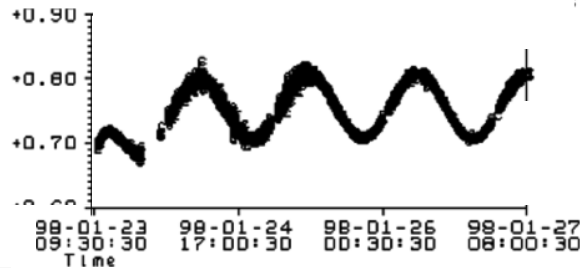
\includegraphics[width = 7.65cm] {Anderson/fig2a_near_doppler_postosc.png}
	};

\node [anchor = north west] (velocitylags) at (0, 0) {
	\begin{tikzpicture}[xscale=0.75,yscale=0.5]
	\begin{axis}[
		scale only axis,
		scaled ticks = false,
		date coordinates in=x,
		date ZERO=1998-01-23,
		xmin={1998-01-23 00:00:00},
		xmax={1998-01-27 09:00:00},
		%xticklabel = {\small{\short{\year}-\month-\day}\\\small{\hour:\minute}},
		xticklabel = {\small{\month-\day}\\\small{\hour:\minute}},
		xticklabel style = {anchor = north, blue, align = center},
		axis x line* = bottom,
		ytick align = outside,
		yticklabel style = {anchor = east, blue},
		every y tick/.style = {blue},
		minor y tick num = 0,
		ytick pos = left,
		axis y line* = left,
		y unit = {1000~\kilo\metre},
		ylabel = {\color{blue}Range},
		ylabel shift = -0.1cm,
		y filter/.code = {\pgfmathparse{1e-6*\pgfmathresult}},
		legend style={
			at = {(0.25,0.25)},
			anchor = west,
			draw = none,
			font = \small,
			fill = none
			}
		]
		\addplot [thick, mark = none, blue]
			table [x index=0, y index=4, col sep=tab, skip first n=1]
			{near_aos.t}
		;
		\addlegendentry[blue] {range $r$};
	\end{axis}
	\begin{axis}[
		scale only axis,
		date coordinates in=x,
		date ZERO=1998-01-23,
		xmin={1998-01-23 00:00:00},
		xmax={1998-01-27 09:00:00},
		xticklabel = \empty,
		xticklabel style = {anchor = north, teal},
		axis x line* = bottom,
		ytick align = outside,
		yticklabel style = {anchor = west, teal},
		ytick pos = right,
		every y tick/.style = {teal},
		minor y tick num = 0,
		ymin = 5.05, %6.6,
		ymax = 7.6,
		y unit = {\kilo\metre/\second},
		ylabel = {\color{teal}Range rate},
		%ylabel style = { rotate = 180 },
		ylabel shift = -0.25cm,
		axis y line* = right,
		y filter/.code = {\pgfmathparse{1e-3*\pgfmathresult}},
		restrict y to domain = 0:10,
		legend style={
			at = {(0.25,0.20)},
			anchor = west,
			draw = none,
			font = \small,
			fill = none
			}
		]
		\addplot [thick, mark = none, teal]
			table [x index=0, y index=5, col sep=tab, skip first n=1]
			{near_aos.t}
		;
		\addlegendentry[teal] {range rate $v$};
	\end{axis}
	\begin{axis}[
		scale only axis,
		date coordinates in=x,
		date ZERO=1998-01-23,
		xmin={1998-01-23 00:00:00},
		xmax={1998-01-27 09:00:00},
		xticklabel = \empty,
		xticklabel style = {anchor = north, violet},
		axis x line* = bottom,
		ytick = \empty,
		yticklabel = \empty,
		ylabel = {},
		y filter/.code = {\pgfmathparse{0.025+\pgfmathresult}},
		restrict y to domain = -0.2:0.1,
		legend style={
			at = {(0.60,0.25)},
			anchor = west,
			draw = none,
			font = \small,
			fill = none
			}
		]
		\addplot [thick, mark = none, violet]
			table [x index=0, y index=6, col sep=tab, skip first n=1]
			{near_aos.t}
		;
		\addlegendentry[violet] {acceleration $a$};
	\end{axis}
	\begin{axis}[
		scale only axis,
		scaled ticks = false,
		date coordinates in=x,
		date ZERO=1998-01-23,
		xmin={1998-01-23 00:00:00},
		xmax={1998-01-27 09:00:00},
		xticklabel = \empty,
		xticklabel style = {anchor = north, red},
		axis x line* = bottom,
		ytick pos = right,
		ytick align = inside,
		yticklabel style = {anchor = west, red},
		yticklabel shift = -1.0cm,
		every y tick/.style = {red},
		minor y tick num = 0,
		y unit = {\milli\metre/\second},
		ylabel = {\color{red}Velocity lag},
		ylabel style = { at = { (ticklabel cs:0.40) } },
		ylabel shift = -1.3cm,
		axis y line* = left,
		y filter/.code = {\pgfmathparse{(-1000*\pgfmathresult)}},
		legend style={
			at = {(0.60,0.20)},
			anchor = west,
			draw = none,
			font = \small,
			fill = none
			}
		]
		\addplot [smooth, mark = none, red]
			table [x index=0, y index=10, col sep=tab, skip first n=1]
			{near_aos.t}
		;
		\addlegendentry[red] {$\Delta v = -ar/c$};

		\addplot [dashed, red] coordinates {
			(1998-01-23 00:00:00, 0.0)
			(1998-01-27 09:00:00, 0.0)
			};

		\addplot [dashed] coordinates {
			(1998-01-23 09:54:00, -0.050)
			(1998-01-23 09:54:00,  0.300)
			};

		\node [rotate = -90, anchor = south] %coordinate, pin = above right:{\small AOS}]
			at (axis cs:1998-01-23 09:54:00, -70) {\small\it AOS Canberra};

		\node [small dot, pin = 85:{\small $11.13~\milli\metre/\second$}]
			at (axis cs:1998-01-23 09:54:00, 11.13) {};

		% for overlay alignment
		\addplot [loosely dotted, blue] coordinates {
			(1998-01-24 17:00:30, -0.050)
			(1998-01-24 17:00:30,  0.300)
			};

		\addplot [loosely dotted, blue] coordinates {
			(1998-01-26 00:30:30, -0.050)
			(1998-01-26 00:30:30,  0.300)
			};

		\addplot [loosely dotted, blue] coordinates {
			(1998-01-27 08:00:30, -0.050)
			(1998-01-27 08:00:30,  0.300)
			};

	\end{axis}
	\end{tikzpicture}
	};
\end{tikzpicture}
\end{document}
